\vfill
\begin{figure}[htb]\centering
  {%
    \setlength{\fboxsep}{7pt}%
    \setlength{\fboxrule}{1pt}%
    \fbox{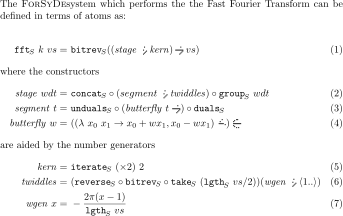
\includegraphics[width=.9\textwidth]{figs/example-forsyde-math}}
  }
\end{figure}
\lstinputlisting{figs/example-forsyde-math.tex}
\vfill
\newpage

\section{The \texttt{forsyde-math} package}
\label{sec:forsyde-math-package}

This package provides a set of symbols and commands for writing equations mainly for the \ForSyDeAtom\ theoretical framework.

\subsection{Symbol Fonts}
\label{sec:fonts}

All \ForSyDeAtom\ operators have been bundled in a font family called \texttt{forsydeatom}, which can be used imported in accordance to the \LaTeXe\ standard. The math symbol font is called \texttt{atomoperators} and it is based on the \texttt{forsydeatom} font family.

The \texttt{forsyde-math} imports these fonts and provides macros for typing them in math or texst environments.

\def\makesymbolrow#1{{\tiny #1} & {\scriptsize #1} & {\footnotesize #1} & {\small #1} & {\normalsize #1} & {\large #1} & {\Large #1} & {\LARGE #1} & {\huge #1} & {\Huge #1}}
\begin{longtable} { c | c c c c c c c c c c }
  \toprule
  \textbf{Command}  & \textbf{5pt} & \textbf{7pt} & \textbf{8pt} & \textbf{9pt} & \textbf{10pt} & \textbf{12pt} & \textbf{14.4pt} & \textbf{17.28pt} & \textbf{20.74pt} & \textbf{24.88pt} \\
  \midrule
  \texttt{\string\BhFun} & \makesymbolrow{\textBhFun} \\
  \texttt{\string\BhApp} & \makesymbolrow{\textBhApp} \\
  \texttt{\string\BhDef} & \makesymbolrow{\textBhDef} \\
  \texttt{\string\BhPhi} & \makesymbolrow{\textBhPhi} \\
  \midrule
  \texttt{\string\MocFun} & \makesymbolrow{\textMocFun} \\
  \texttt{\string\MocApp} & \makesymbolrow{\textMocApp} \\
  \texttt{\string\MocCmb} & \makesymbolrow{\textMocCmb} \\
  \texttt{\string\MocPre} & \makesymbolrow{\textMocPre} \\
  \texttt{\string\MocPhi} & \makesymbolrow{\textMocPhi} \\
  \texttt{\string\MocDel} & \makesymbolrow{\textMocDel} \\
  \midrule
  \texttt{\string\SkelFrm} & \makesymbolrow{\textSkelFrm} \\
  \texttt{\string\SkelPip} & \makesymbolrow{\textSkelPip} \\
  \texttt{\string\SkelFun} & \makesymbolrow{\textSkelFun} \\
  \texttt{\string\SkelApp} & \makesymbolrow{\textSkelApp} \\
  \texttt{\string\SkelRed} & \makesymbolrow{\textSkelRed} \\
  \texttt{\string\SkelRec} & \makesymbolrow{\textSkelRec} \\
  \bottomrule
\end{longtable}


%%% Local Variables:
%%% TeX-command-default: "Make"
%%% mode: latex
%%% TeX-master: "../refman"
%%% End:
